\section{Introduction}
In this chapter, we will address SLAM (simultaneous localization and mapping) and navigation techniques used in this thesis. We will focus exclusively on the literature overview of techniques used in practice, without comparing the various existing approaches. We will therefore overview all the components of the see-plan-act architecture.
The sense-plan-act architecture in fact explains the entire process that starts from the map building, to the global and local planning up to sensor fusion.
It is indeed composed of:
\begin{itemize}
    \item Map
    \item Sensors 
    \item Current Position
    \item Goal Position
    \item Trajectory Planning
    \item Trajectory Following and Obstacle Avoidance
\end{itemize}

\begin{figure}[H]
    \centering
    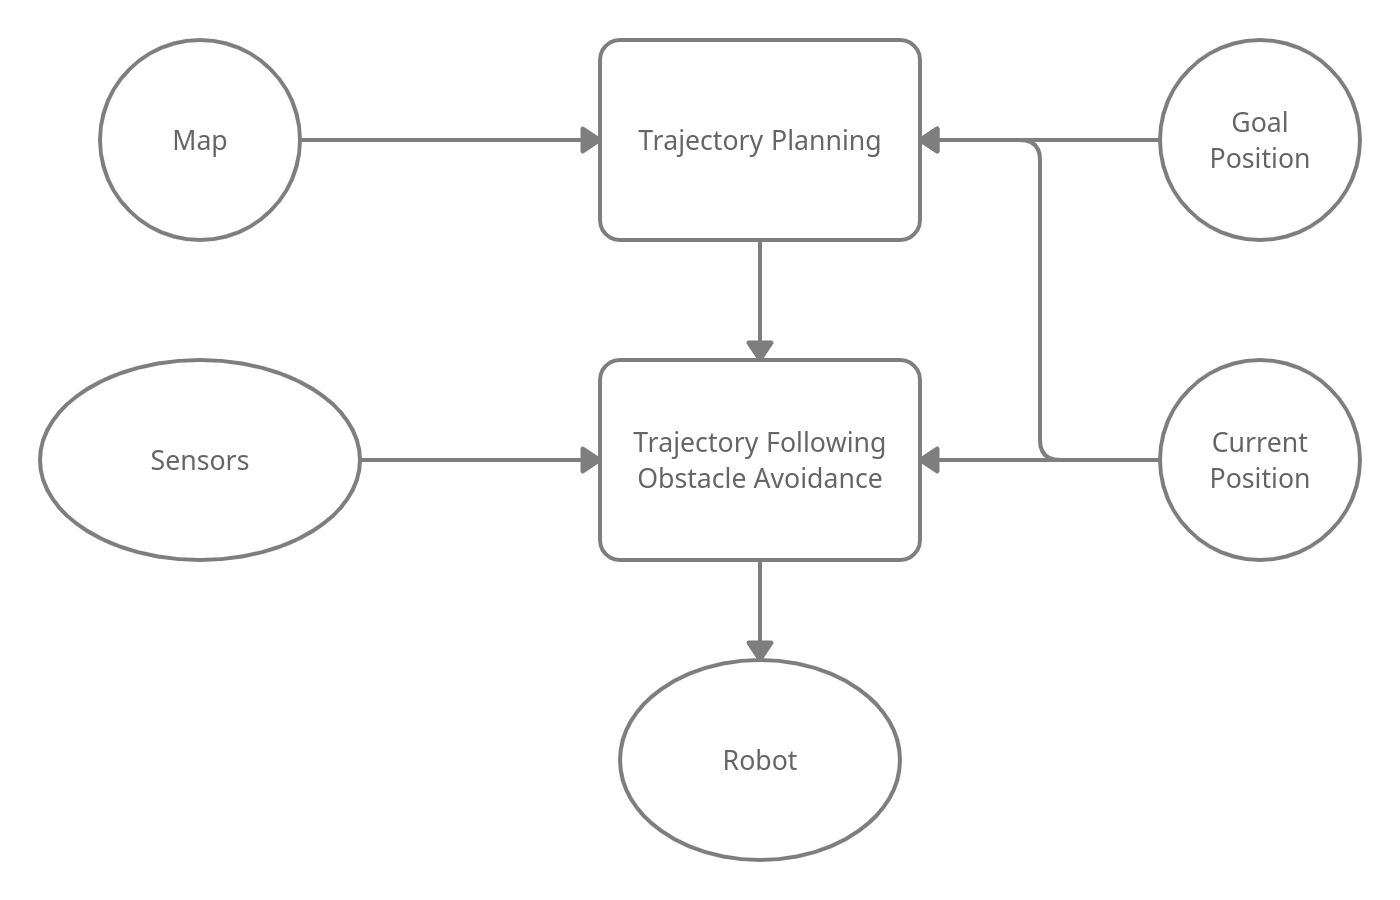
\includegraphics[scale=0.21]{Images/Chapter 4/senseplanact.png}
    \caption{Block scheme representation of sense plan act architecture}
    \label{fig:my_label}
\end{figure}

\section{Simultaneous Localization and Mapping}
In this first subsection we will focus on map side, understanding how maps are build, interpreted and how the agents localize inside the map. There exists two main types of representing a map:
\begin{itemize}
    \item Landmark-based: a particular type of representation, mainly used for localization, that is based on detecting landmarks. This technique results in a sparse representation of the space, leaving much to the unknown;
    \item Grid maps: the map results in a discredited version of the environment, where each cell contain information about occupation/non occupation/unkwown. It results in a very dense representation where almost the totality of the cells are caught.
\end{itemize}

In the scope of this work we will focus on occupancy grid map.
\subsection{Occupancy Grid Map}
As anticipated, occupancy grid map is a peculiar map representation that attempts to discretize the continous environment into a two dimensional grid map. The grid map is again divided into array cells of size from 5 to 50 cm and each of them hold a probability value that stands for the likelihood to be free or occupied.
Thus, occupancy grid maps try to solve the problem of reconstructing consistent maps from noisy and uncertain measurement data, under the hypothesis of knowing the robot pose. 
The reasoning behind most occupancy grid mapping algorithm is to calculate the posterior over maps, given the data, in a probabilistic way.
\begin{equation}
    p(m | z_{1:t},x_{1:t})
\end{equation}
where m is the map,$z_{1:t}$ is the set of measurements up to time t and $x_{1:t}$ the set of all the poses taken by the robot, namely its path.
Being $m_{i}$ the i-th grid cell and having it a binary occupancy value that states if a cell is free or occupied (1 for the cell being occupied, 0 free), we can define:
\begin{equation}
m = \sum_{i}^{}{m_{i}}    
\end{equation}.
\begin{figure}[H]
    \centering
    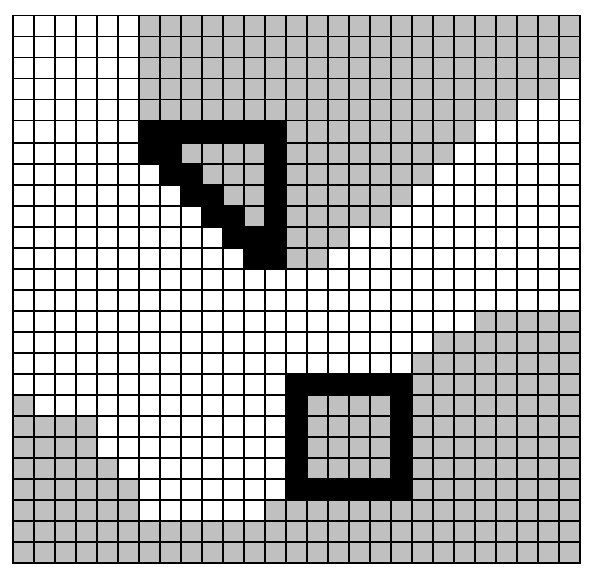
\includegraphics[scale=0.5]{Images/Chapter 4/occupancygrid.png}
    \caption{Sample of an Occupancy Grid}
    \label{fig:occupancygrid}
\end{figure}
Due to the curse of dimensionality, the probabilistic approach reduces to estimate the single cell occupancy rather than the entire map:
\begin{equation}
    p(m_{i} | z_{1:t},x_{1:t})
\end{equation}

To calculate the single cell occupancy we resort to Bayes rule:
\begin{equation}
    p(m_{i} | z_{1:t},x_{1:t}) = \frac{p(z_{t} | m_{i},z_{1:t-1},x_{1:t}) p(m_{i} | z_{1:t-1},x_{1:t})}{p(z_{t} |z_{1:t-1},x_{1:t})}
\end{equation}

Additionally recurring to Markov assumption, stating that the current state depends on only a finite fixed number of previous states, measurement $z_{t}$ depends only on $x_{t}$ and $m_{i}$.
It is common use at this point to adopt log-odds representation of occupancy, as to avoid being with probabilities close to 0 and 1:
\begin{equation}
    l_{t,i} = \log{\frac{p(m_{i} | z_{1:t},x_{1:t})}{1 - p(m_{i} | z_{1:t},x_{1:t})}}
\end{equation}

The process loops and assumes the form of the algorithm \ref{alg:occupancy}.
It is important to note that only the cells which fall under the sensor cone of measurement are updated through the inverse sensor model, \citet{thrun2005probabilistic}.
\begin{algorithm}
\caption{Occupancy Grid Algorithm}\label{alg:occupancy}
\begin{algorithmic}
\STATE Algorithm occupancy grid mapping({$l_{t-1,i},x_{t},z_{t}$})
\FOR{all cells $m_{i}$}
    \IF{$m_{i}$ in perceptual field of $z_{t}$}
        \STATE $l_{t,i}$ = $l_{t-1,i}$ + $inverse\_sensor\_model(m_{i},x_{t},z_{t} - l_{0})$
    \ELSE
        \STATE $l_{t,i}$ = $l_{t-1,i}$
    \ENDIF
\ENDFOR
\RETURN  {$l_{t,i}$}
\end{algorithmic}
\end{algorithm}

where the inverse sensor model is defined as follows:
\begin{equation}
    inverse\_sensor\_model(m_{i},x_{t},z_{t}) = p(m_{i}|z_{t}, x_{t})
\end{equation}
The motivation for the "inverse" denomination is because it reasons from effects to causes: it provides an information about the world where that same information was derived from a measurement caused by the world it self:

\begin{equation}
    p(m_{i} | z_{1:t},x_{1:t}) = \eta \int{m:m(i)=m_{i}}^{} p(z | x,m) p(m) dm
\end{equation}

A function approximator has to be used, since this algorithm cannot be computed due to the large map space.

\subsection{SLAM algorithm}
At this point we turn to the problem of SLAM, Simultaneous Localisation and Mapping. This stems from the robot's need to map a new environment, of which nothing is known, and at the same time to localise the robot itself within the map being created. The problem is particularly difficult as one does not have access to the robot's poses and uncertainty is kept on all the components.
Moreover, it proposes to correct both odometry and uncertainty of estimated position and landmark.
Two approaches to SLAM can be defined, from a probabilistic point of view:
\begin{itemize}
    \item Full SLAM: simultaneous estimate of path and map
    \item Online SLAM: simultaneous estimate of the most recent pose and map
\end{itemize}

\textbf{Full SLAM}
Full SLAM addresses the problem of estimating the joint probability of the entire trajectory and landmark.
\begin{equation}
    p(x_{1:t}, m | z_{1:t},u_{1:t})
\end{equation}
For this purpose we propose a significant example: FastSLAM.
Fast Simultaneous Localization and Mapping uses a sampled particle filter distribution model, solving the full SLAM problem.
If we consider the full trajectory $X_{t}$ rather than a single pose $x_{t}$, the following holds:
\begin{equation}
    p(X_{t}, m | z_{t}) = P(X_{t}| z_{t}) P(m | X_{t}, z_{t})
\end{equation}
where $P(X_{t}| z_{t})$ is the estimate of the trajectory and $P(m | X_{t}, z_{t})$ is the estimate of the map given the trajectory.
Thus, in FastSLAM the trajectory $X_{t}$ is represented by particles $X_{t}(i)$ while the map is represented by a factorization called Rao-Blackwellized filter.
The approach so is to treat each pose particle as it it was the entire trajectory, processing all of the feature measurements independently.

\begin{equation}
    P(m | X_{t}^{(i)},z_{t}) = \prod_{j}^{M} P(m_{j} | X_{t}^{(i)},z_{t})
\end{equation}
Indeed, once the trajectory is known, all of the features become uncorrelated.

\begin{equation}
    p(x_{1:t},l_{1:m} | z_{1:t},u_{0:t-1}) = p(x_{1:t} | z_{1:t},u_{0:t-1})p(l_{1:m} | x_{1:t},z_{1:t}) 
\end{equation}
where we have SLAM posterior, robot path posterior and landmark positions respectively. Previous equation can be simplified by factorization as follows:

\begin{equation}
     p(x_{1:t},l_{1:m} | z_{1:t},u_{0:t-1}) = p(x_{1:t} | z_{1:t},u_{0:t-1})\prod_{i=1}^{M}p(l_{i} | x_{1:t},z_{1:t})
\end{equation}
In this way the dimension of state space is reduced making particle filtering possible:
\begin{equation}
    O(N\times\log(M))
\end{equation}
with N being the number particles and M the number of map features
\begin{figure}[H]
    \centering
    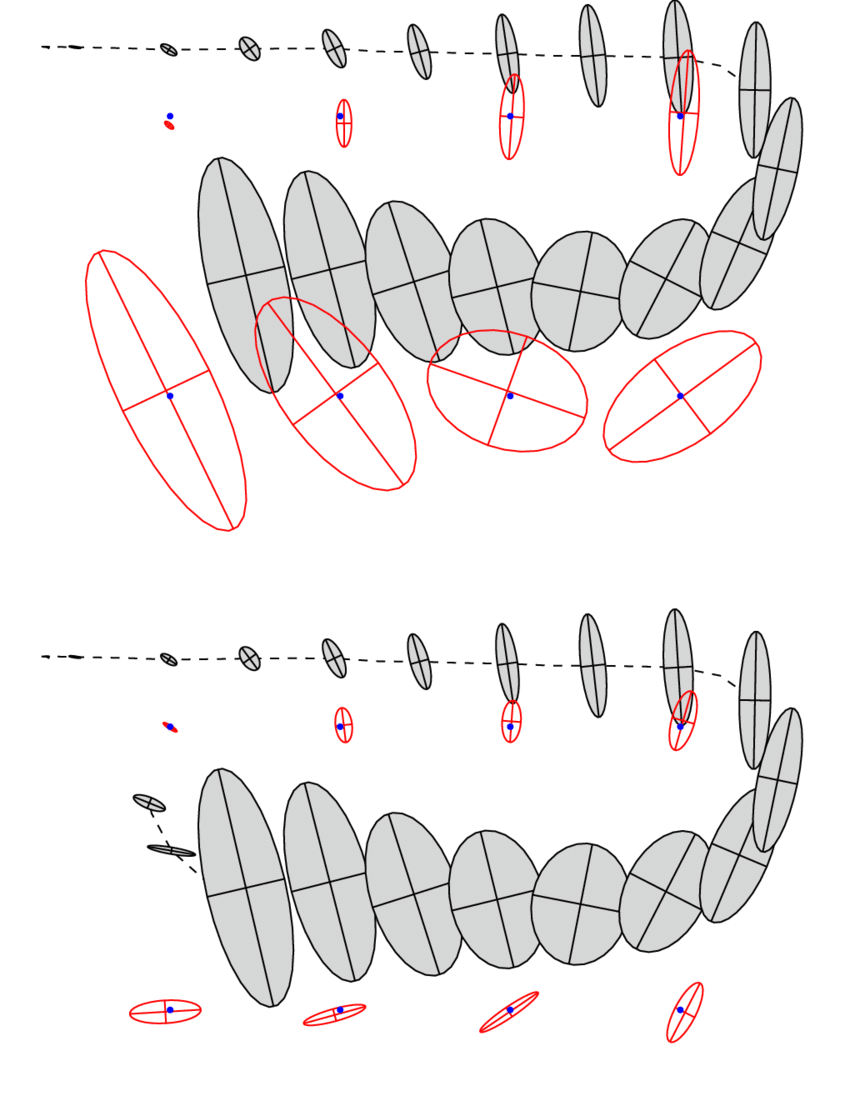
\includegraphics[scale=0.34]{Images/Chapter 4/slam_uncertainty.png}
    \caption{SLAM problem: initial uncertainty on pose and consequent decrease thanks to previously seen landmarks, \citet{thrun2004}}
    \label{fig:slam_uncertainty}
\end{figure}
Summarizing, FastSLAM adopts a Rao-Blackwellized particle filtering based on landmarks, \citet{montemerlo2002}, where each particle is a trajectory, each landmark is represented by a 2x2 EKF and therefore each particle has to maintain M EKFs.



\textbf{Online SLAM}
Online SLAM entails estimating the posterior over the last pose along with the map:
$p(x_{t},m_{i} | z_{1:t},u_{1:t})$ where $x_{t}$ is the pose at time t, m is the map, $z_{1:t}$ $u_{1:t}$ the measurements available up to time t.
The fact that we refer to this technique as online SLAM directly derives from the fact that we're considering data at time t, estimating last pose only.
\begin{equation}
    p(x_{t}, m | z_{1:t},u_{1:t}) = \int \int ... \int{}^{} p(x_{1:t}, m | z_{1:t}, u_{1:t}) dx_{1}dx_{2} ... dx_{t-1}
\end{equation}
As one can notice, the online SLAM problem is the result of integrating out one at a time past poses from the full SLAM problem.
A significant example of a proposed solution to Online SLAM is proposed: EKF SLAM.
Extended Kalman Filter Simultaneous Localization and Mapping uses a linearized Gaussian probability distribution.


\begin{algorithm}
\caption{Extended Kalman Filter}\label{alg:ekf_slam}
\begin{algorithmic}
\STATE Extended Kalman filter({$\mu_{t-1},\Sigma_{t-1},u_{t},z_{t}$})
\STATE {$\mu$}' = g($u_{t}$, $\mu_{t-1}$)
\STATE $\Sigma_{t}^{}$' = $G_{t}\Sigma_{t-1}^{} G_{t}^{T} + R_{t}$
\STATE $K_{t}$ = $\Sigma_{t}'H_{t}^{T}(H_{t}\Sigma_{t}'H_{t}^{T} + Q_{t})^-1$
\STATE $\mu_{t}$ = $\mu_{t}' + K_{t}(z_{t} - h{\mu_{t}})$
\STATE $\Sigma_{t}$ = $(I - K_{t}H_{t})\Sigma_{t}'$
\RETURN $\mu_{t}, \Sigma_{t}$
\end{algorithmic}
\end{algorithm}

EKF-SLAM promises good performances but it has two main drawbacks: it employs linearized models of non-linear motion and observation models, inheriting many caveats; it is computationally demanding.
One possible solution to this problem is the above reported FastSLAM (Rao-Blackwellisation filter).

\subsection{SLAM Toolbox}
During the experience at Oversonic Robotics, the SLAM toolbox was chosen for the simultaneous localisation and mapping problem, though many predecessors exist.
The ROS packages responsible of SLAM can be divided into Bayes-based filter implementations, like GMapping and HectorSLAM, and graph-based implementations, as Cartographer and Karto SLAM.
The SLAM Toolbox package is an open source software developed by Steve Maceski which use graph based approach and occupancy grid map.
It has been widely used on the various ROS distros and has become the default SLAM algorithm for ROS2. It arose from the need to build accurate maps of large environments, where previous SLAM tools had shown shortcomings.\\
SLAM Toolbox provides three operating modes, \citet{Macenski2021}:
\begin{itemize}
    \item Synchronous Mapping: provides the ability to map and localize in an environment while keeping a bunch of measurements to be added to SLAM. This results useful when the quality of the map is important.
    \item Asynchronous Mapping: on the contrary, this mode manages new measurements only when previous measurement has been completed. This makes this modality useful when real time localization is crucial.
    \item Pure Localization: cannot detects changes in the space. It tries to match a local bunch of measurements with the data originally gathered.
\end{itemize}

\subsection{Advanced Monte Carlo Localization}
The pose estimation used in Oversonic applications is based on AMCL pose (Advanced Monte Carlo Localization). 
This technique relies on the so called particle filter approach. An extremely large number of particles covering the entire state space are used to initialize particle filters. The robot has a multi-modal posterior distribution because it predicts and update the measurements as it obtains more measurements. A Kalman Filter approximates the posterior distribution to be a Gaussian, which is a significant departure from this. The particles converge to a single value in state space after several rounds. Maintaining the random distribution of particles over the state space is a major challenge for particle filters, which becomes impossible for large dimensional problems. These factors make an adaptive particle filter far superior to a simple particle filter in terms of convergence speed and computational efficiency. 
\begin{figure}[H]
    \centering
    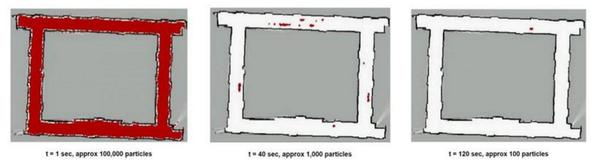
\includegraphics[scale=0.5]{Images/Chapter 4/amclocalization.png}
    \caption{Particle Filter in Action over Progressive Time Steps, \citet{amclimage}}
    \label{fig:amclpart}
\end{figure}The main concept is to limit the inaccuracy caused by the particle filter's sample-based representation. The real posterior is thought to be represented by a discrete, piecewise constant distribution, such as a discrete density tree or a multidimensional histogram, in order to calculate this bound. We start with a map of our surroundings when using an adaptive particle filter for localization, and we can either manually localize the robot by setting it to a certain point or we may make the robot start from with no initial estimate of its position. We now create new samples that forecast the robot's position following the motion command as it advances. By re-weighting these samples and leveling the weights, sensor readings are included. In general, it is a good idea to add a few random, evenly dispersed samples because they aid in the robot's recovery when it loses track of its location. Without these random samples, the robot will continue to resample from the erroneous distribution under those circumstances and will never recover. We could encounter dis-ambiguities inside a map due to symmetry in the map, which is what gives us a multi-modal posterior belief, which is why it takes the filter many sensor readings to converge.

\section{Global Planning}
Mobile robots are meant to move from their current positions to some goal inside the map.
Once that the SLAM task has been performed and a map has been obtained, we can address the This is known as trajetory planning and it is managed by the so-called global planner.
Robot motion planning goals are:
\begin{itemize}
    \item collision-free trajectories
    \item most efficient or most optimal (depending on the chosen optimality criterion) trajectory
\end{itemize}
The problem that global planner addresses regards finding a collision free path between an initial pose and the goal, taking into account the existing constraints.
It is important to distinguish between some concepts used in this scope:
\begin{itemize}
    \item Path: a geometric locus of way points
    \item Trajectory: a path for which a temporal law is specified
    \item Manouver: a series of actions that a vehicle should execute
\end{itemize}

In the scope of this thesis we are going to analyze a path planning algorithms, the so-called A*.
This algorithms is part of the graph based planning family.
The underlying idea is to construct a discretized representation of the map, building a graph out of it (4 or 8 neighbors connectivity are possible) and eventually searching for the shortest path in the graph, namely the optimal solution. It is relevant to report that the resolution of the grid directly influences the accuracy of the plan: a more dense resolution will describe in a more complete way the map it is investigating, thus resulting in a deeper analysis of the possible paths.

\begin{figure}[H]
     \centering
     \subfloat[][a]{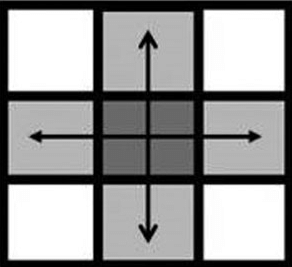
\includegraphics[scale=0.45]{Images/Chapter 4/4connectivity.png}\label{4 connectivity}}
     \hfill
     \subfloat[][b]{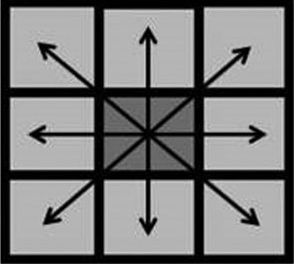
\includegraphics[scale=0.46]{Images/Chapter 4/8connectivity.png}\label{8 connectivity}}
     \caption{Comparison of 4 connectivity (a) and 8 connectivity (b)}
     \label{steady_state}
\end{figure}
This connectivity scheme reproduces on a grid the kinematics motion a robot is supposed to do in reality, so that performing the path search on the grid is representative of how the robot would move in reality. 
The usual approach to search graphs for the optimal path 
\subsection{A* algorithm}
The A* algorithm was developed on the basis of the Dijkstra algorithm m improving its performance and is therefore one of the most widely used in path finding and graph traversal today.
The components of this algorithm are the two points (start and end point), the grid and the nodes. 
In this approach what is important is the cost of moving from one edge to the others.
The predecessor of A*, Dijkstra algorithm, in fact focuses on the idea of cost: each part of the path has an intrinsic cost and the algorithm visits all of the existing edges trying to lower the overall cost. The algorithm manages a queue list where it keeps all the nodes that are still to analyzed, where the nodes with the smallest distance to the starting point is the first node in the queue, \citet{herzog}.
Every time we move to some node, we encounter other nodes that previously were unaccessible, since we are dealing with k connectivity framework, and if these nodes are still to be traversed they are added to queue. This process ends as soon as the priority queue is emptied, namely when there are no nodes left to be investigated.
Every time the algorithm shifts to some new node it records the path that led to that node and the specific costs, so the shortest path to each node can be computed by going backwards in the path.
A* is based on the best first search speeds up this process by splitting the cost into a function:
\begin{equation}
    f(x) = g(x) + h(x)
\end{equation}

where g(x) is cost of the shortest path from the starting point to the current node and h(x), the so-called heuristic function, is an estimate of the cost of the shortest path from the current state to the goal.
The kind of heuristic is a matter of choice, still it needs to comply with the following three properties:
\begin{itemize}
    \item Completeness: the algorithm is guaranteed to terminate when dealing with finite graphs having non negative edge weights.
    \item Admissibility: the heuristic never overestimates the cost of reaching the goal.
    \newpage
    \begin{equation}
        h(x) \le h^*(x)
    \end{equation}
    where h*(x) is defined as the optimal cost to reach a goal from the current node.
    
    \item Consistency: the estimate of the algorithm is always less than or equal to the estimated distance from any neighbouring node to the goal, plus the cost of reaching that node.
\end{itemize}
Time complexity strongly depends on the heuristic and in its worst case (the case in which the search space is unbounded), the number of nodes exploded is exponential in the depth of the solution:
\begin{equation}
    d: O(b^d)
\end{equation}
where b is defined as the branching factor.
In its best case (the search space is a tree and there exists only one goal) it would develop in a polynomial fashion, provided that the following condition on the heuristic holds:
\begin{equation}
    |h(x) - h^*(x)| = O(\log{h^*(x)})
\end{equation}
where h* is the optimal heuristic.
For this reason, a bounded relaxation is applied: it is possible to speed up the process by considering also approximate shortest paths. This process is bounded by a factor $\epsilon$ so that optimality  suffers a decrease that is not greater than (1 + $\epsilon$) times the optimal solution, computed without the hypothesis relaxation.
Several possible algorithms exists for $\epsilon$, below is reported as an example the Dynamic Weighting, \citet{10.5555/1624775.1624777}:\\
cost function is defined as
\begin{equation}
    f(n) = g(n) + (1 + \epsilon w(n))h(n)
\end{equation}
where w(n) is
\begin{equation}
    w(n) = 
    \begin{cases}
1 - \frac{d(n)}{N}, & \text{if}\ d(n) \le N \\
0 , & \text{otherwise}
\end{cases}
\end{equation}
with d(n) being the depth of the search and N the anticipated length of solution.
Below is reported the pseudocode of the $A^{*}$ algorithm:

\begin{algorithm}
\caption{A algorithm}\label{alg:a_star}
\begin{algorithmic}
\STATE Input: A graph G(V,E) with source node start and goal node end
\STATE Output Least cost path from start to end
\STATE open\_list = {start}
\STATE closed\_list = {}
\STATE g(start) = 0
\STATE h(start) = heuristic\_function(start,end)
\STATE f(start) = g(start) + h(start)
\WHILE{open list is not empty}
    \STATE m = Node on top of open\_list, with least f
    \IF{m == end}
        \RETURN
    \ENDIF
    \STATE remove m from open\_list
    \STATE add m to closed\_list
    \FOR{each n in child(m)}
    \IF{n in closed\_list}
    \STATE continue
    \ENDIF
    \STATE cost = g(m) + distance(m,n)
    \IF{n in open\_list and cost < g(n)}
    \STATE remove n from open list as new path is better
    \ENDIF
    \IF{n in closed\_list and cost < g(n)}
    \STATE remove n from closed list
    \ENDIF
    \IF{n not in open\_list and n not in\_closed list}
    \STATE add n to open\_list
    \STATE g(n) = cost
    \STATE h(n) = heuristic\_function(n, end)
    \STATE f(n) = g(n) + h(n)
    \ENDIF
    \ENDFOR
    \ENDWHILE
\RETURN failure
\end{algorithmic}
\end{algorithm}
It is interesting to note that the algorithm returns either the optimal plan, hence it is an exact algorithm.
\begin{figure}[H]
    \centering
    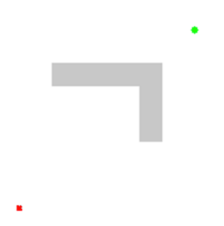
\includegraphics[scale=0.60]{Images/Chapter 4/Aproblem.png}
    \caption{A* initial problem: red point is the starting node, green point is the goal}
    \label{fig:aproblem}
\end{figure}

\begin{figure}[H]
     \centering
     \subfloat[][a]{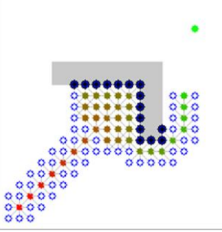
\includegraphics[scale=0.60]{Images/Chapter 4/Asol1.png}\label{}}
     \hfill
     \subfloat[][b]{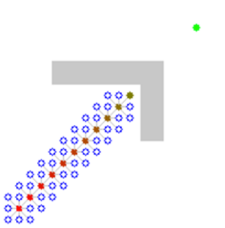
\includegraphics[scale=0.60]{Images/Chapter 4/Asol2.png}\label{}}
     \hfill
     \subfloat[][c]{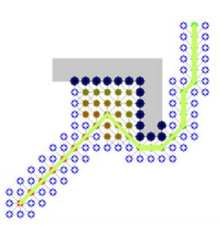
\includegraphics[scale=0.60]{Images/Chapter 4/Asol3.png}\label{}}
     \caption{Shortest path relaxing the admissibility criteria}
     \label{a_sol}
\end{figure}
\begin{figure}[H]
     \centering
     \subfloat[][a]{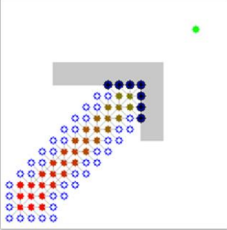
\includegraphics[scale=0.60]{Images/Chapter 4/Arel_sol1.png}\label{}}
     \hfill
     \subfloat[][b]{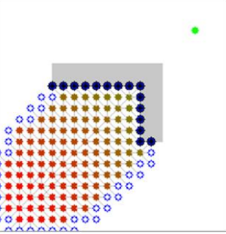
\includegraphics[scale=0.60]{Images/Chapter 4/Arel_sol2.png}\label{}}
     \hfill
     \subfloat[][c]{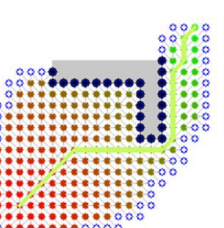
\includegraphics[scale=0.60]{Images/Chapter 4/Arel_sol3.png}\label{}}
     \caption{Optimal path obtained using the admissibility criteria. }
     \label{a_sol}
\end{figure}
\section{Local Planning}
A strong assumption on which global planning technique was based is the fact that the space surrounding the robot from its starting point to its goal is almost totally known. Nonetheless, robots moving in every environment must be able to deal with unforeseen changes and adapt to them. For this purpose, a local planner is paired with the global planner: while the latter is responsible of trajectory planning and  works at a low frequency rate, the first one deals with trajectory following and obstacle avoidance at a much higher frequency rate.
So, local planning is deemed to solve two tasks:
\begin{itemize}
    \item Ensure path following
    \item Perform obstacle avoidance for objects that are not tracked in the map
\end{itemize}
\textbf{Obstacle Avoidance}
“Let A be the robot moving in the workspace W, whose configuration space is CS. Let
q be a configuration, $q_{t}$ this configuration in time t, $A(q_{t}) \in W$ the space occupied by the robot in this configuration.
If in the vehicle there is a sensor, which in qt measures a portion of the space $S(q_{t}) \subset W$ identifying a set of obstacles $O(q_{t}) \subset W$. Let u be a constant control vector and $u(q_{t})$
this control vector applied $q_{t}$ during time $\delta t$. Given $u(q_{t})$, the vehicle describes a trajectory \\
$q_t + \delta_t = f(u, q_t, \delta t)$, with        $\delta t \geq 0$.
Let $Q_t,T$ be the set of the configuration of the trajectory followed from $q_t$ with $\delta t \in (0,T)$ a given time interval. T > 0 is called the sampling period. Indicating with $q_target$ a target configuration. Then, in time $t_i$ the robot A is in $q_ti$, where a sensor measurement is obtained $S(q_{ti})$, and thus an obstacle description $O(q_ti)$.” \citet{SicilianoKhatib2008}
The overall goal of the obstacle avoidance algorithm is to find a trajectory from that brings the robot closer to the goal in a non colliding way:\\
$A(q_{ti}, T) \cap O(q_ti) = \emptyset$ \\
$f(q_{ti}, q_{target}) \le F(q_{ti} + T, q_{target})$\\
\begin{figure}[H]
    \centering
    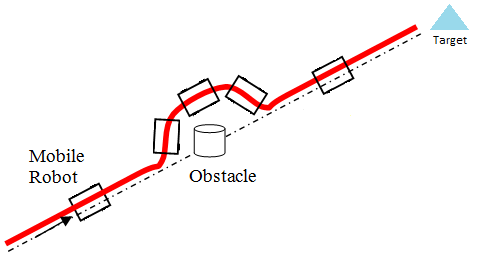
\includegraphics[scale = 0.5]{Images/Chapter 4/obstacleavoidance.png}
    \caption{Sample of the most simple obstacle avoidance technique}
    \label{fig:obstacleavoidance}
\end{figure}
In the following subsections an overview of the most famous local planning method will be provided, in particular:
\begin{itemize}
    \item Vector Field Histogram
    \item Curvature Velocity
    \item Dynamic Window Approach
\end{itemize}
\subsection{Vector Field Histograms}
Vector Field Histogram was presented in 1991 by \citet{borenstein1991} and ensured fast obstacle detection and collision avoidance, not requiring the vehicle to stop. It is composed of two steps, where the first one all the possible motions are evaluate and in the second one the best one is traversed.
    \begin{figure}[H]
        \centering
        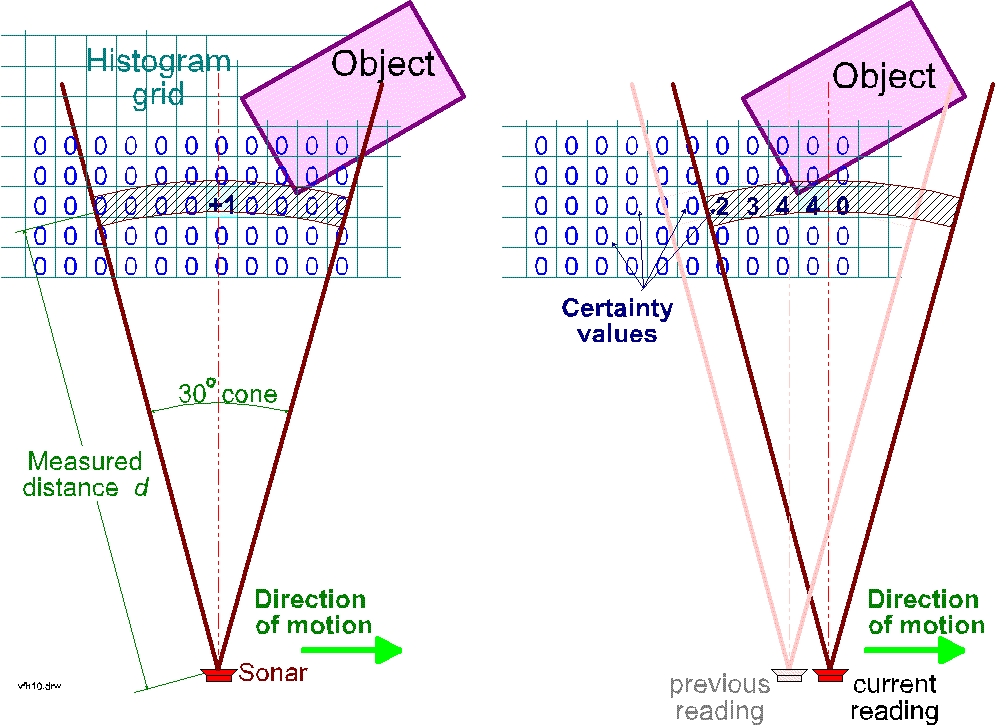
\includegraphics[scale=0.30]{Images/Chapter 4/vff1.png}
        % \hfill
        % \subfloat[]{}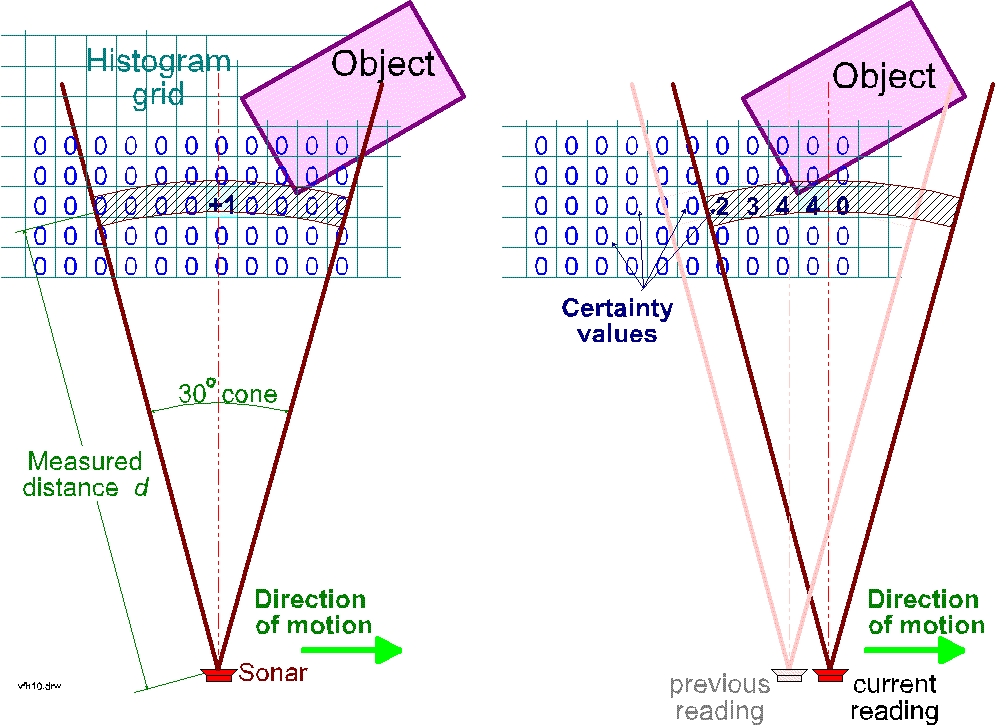
\includegraphics[scale=0.25]{Images/Chapter 4/vff2.png}
        \caption{Vector Field Histogram}
        \label{fig:my_label}
    \end{figure}
The Vector Field Histogram is based on the concept of virtual force field, a concept that resort somehow to the idea of imaginary forces acting on a robot, \citet{1087247}.
VFF is composed of:
\begin{itemize}
    \item A two-dimensional Cartesian histogram grid for obstacle representation, where the grid is composed of cells defined by some coordinate (i,j) and $c_{i,j}$ holds the probability of the occupancy. A probability distribution is created by updating only one cell in the histogram grid for each range reading.
    More specifically, the function $h^k(q_{ti})$ describes the density of the obstacle, on turn proportional to the probability of point occupancy P(p) and to distance from the obstacle, that is to say that the more the distance increases, the lower is the density.
    The function $h^k(q_{ti})$ is defined as:
    \begin{equation}
        h^k(q_{ti}) = \int_{\Omega_k} P(p)^n\left(1 - \frac{d(q_{ti},p)}{d_{max}}\right)^m dp
    \end{equation}
    \begin{figure}[H]
        \centering
        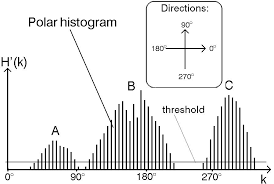
\includegraphics{Images/Chapter 4/potentialfield.png}
        \caption{Vector Field Histogram}
        \label{fig:my_label}
    \end{figure}
    \item Application of potential field idea to the histogram grid
    \item Previous two component are combined in real time enables sensor data to perform obstacle avoidance
\end{itemize}
All the directions ranged from the sensors are evaluated but only those that fall under the defined threshold are further investigated. A cost function is then established as follows:
\begin{equation}
    G = \alpha \times target\_direction + \beta \times  wheel\_orientation + \gamma \times previous\_direction
\end{equation}
where $\alpha$ represents the direction of the goal, $\beta$ the smoothing of the action and $\gamma$ the previous direction of motion.
Every direction, falling under the threshold, is evaluated through the newly defined cost function, that becomes the selection method.

\subsection{Curvature Velocity Methods}
Curvature Velocity Methods were developed by Reid Simmons in 1996.
This approach to obstacle avoidance treats the problem as a constrained optimization in the velocity space of the robot, rather than in Cartesian space.
The robot is deemed to travel along arcs of circles rather than straight lines, still it cannot turn instantaneously.
This method works by adding constraints to the velocity space, defined as the set of controllable velocities and choosing the point in that space that complies with all the constraints and maximizes an objective function, that balances speed, safety and goal-directedness, \citet{simmons}.
\begin{figure}[H]
    \centering
    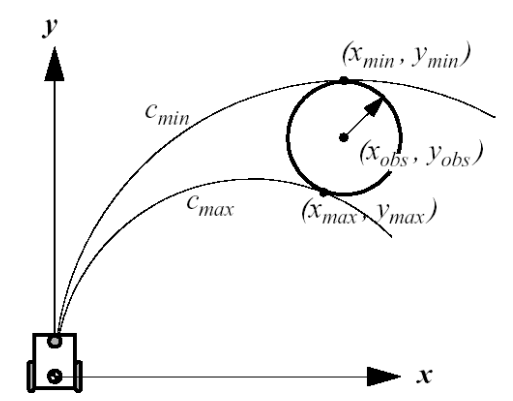
\includegraphics[scale= 0.5]{Images/Chapter 4/vcm.png}
    \caption{Curvature Velocity Methods}
    \label{fig:cvm}
\end{figure}
Only the interval of curvatures between $c_{min}$ and $c_{max}$ are considered, where the set of considered trajectories is obtained by using the curvatures tangent to obstacles to divide the velocity space  into regions of constant distance.

\newpage
\subsection{Dynamic Window Approach}
The dynamic window approach is an obstacle avoidance technique developed by Dieter Fox, Wolfram Burgard and Sebastian Thrun in 1997. 
In the DWA approach, the search for commands to control the robot takes place directly in velocity space. Compared to the previously seen method, the robot's dynamics are also integrated, thus further constraining the velocity search space to those that respect the dynamics constraints and are safe with respect to the obstacle.
The process can be divided into search space and optimization, \citet{fox1997}.
The search space of the possible velocities is reduced in three points:
    \begin{itemize}
        \item Circulare Trajectories: only circular trajectories are considered, determined by pair of (v,w) translational and rotational velocities
        \item Admissible Velocities: restriction to consider only safe velocities
        \item Dynamic Window: further restriction that applies to the admissible velocities, selecting only those that can be reached within a short time interval, respecting the constraints on acceleration.
    \end{itemize}
The dynamic windows search space reduces to $V_r = V_s \cap V_a \cap V_d$\\

Optimization step proposes to maximize the objective function
\begin{equation}
    G(v,w) = \sigma(\alpha \times heading(v,w) + \beta \times dist(v,w) + \gamma \times vel(v,w))
\end{equation}
where \textit{heading} is a measure of progress towards goal location, \textit{dist} is the distance towards the closest obstacle and \textit{vel} is the the foward velocity of the robot.
\begin{figure}[H]
    \centering
    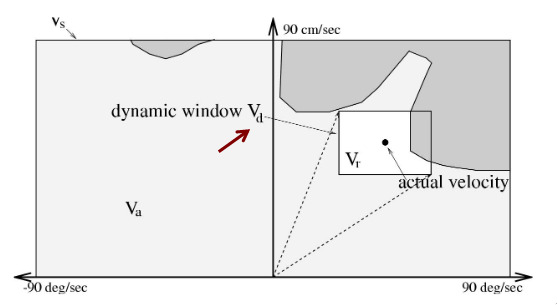
\includegraphics[scale=0.75]{Images/Chapter 4/dynamic_window.jpg}
    \caption{Dynamic Window}
    \label{fig:dwa}
\end{figure}

\begin{algorithm}
\caption{DWA algorithm}
\begin{algorithmic}
\STATE BEGIN DWA(robotpose, robotGoal, robotModel)
\STATE desired\_V = calculate\_V(robotPose,robotGoal)
\STATE   laserscan = readScanner()
\STATE   $allowable_v$ = generateWindow(robot\_V, robotModel)
\STATE   $allowable_w$  = generateWindow(robot\_W, robotModel)
\FOR{each v in $allowable_v$}
      \FOR{for each w in $allowable\_w$}
      \STATE dist = $find\_dist$(v,w,laserscan,robotModel)
      \STATE breakDist = calculateBreakingDistance(v)
      \IF{(dist > breakDist)}  
         \STATE heading = hDiff(robotPose,goalPose, v,w)
         \STATE clearance = (dist-breakDist)/(dmax - breakDist)
         \STATE cost = costFunction(heading,clearance, $abs(desired\_v - v)$)
         \IF{(cost > optimal)}
            \STATE $best\_v = v$
            \STATE $best\_w = w$
            \STATE optimal = cost
        \ENDIF
      \ENDIF
      \ENDFOR
\ENDFOR
\STATE  set robot trajectory to $best\_v, best\_w$
\END
\end{algorithmic}
\end{algorithm}
\newpage
